\section{Detector validation: how far does reconstruction go?}
\label{sec:howfar}
Every number in this section comes from \benchname{} subjects whose ground truth was
recorded from the loaded configs.  Detectors and thresholds were frozen before any label
was analysed.  Table~\ref{tab:accuracy} is the paper's central empirical object.
Table~\ref{tab:matrix} is its one-look summary: for each observable channel, the
property it bears on, its identifiability class, its measured accuracy, and the main
thing that can fool it.

\begin{table}[!htb]\centering\footnotesize
\caption{The observability matrix: what each API channel can establish about the hidden
system, measured on \benchname{}.  \textbf{Class} is the boundary label of
Sec.~\ref{sec:ident}: \textbf{I} identified, \textbf{C} cost-limited ($\hat\kappa$
priced), \textbf{A} access-limited (channel absent or weak here), \textbf{N}
non-identifiable (witness).  Accuracy is top-1 against ground truth.}
\label{tab:matrix}
\begin{tabularx}{\textwidth}{@{}p{1.9cm} p{2.5cm} c p{2.2cm} p{2.6cm} Y@{}}
\toprule
\textbf{Channel} & \textbf{Property} & \textbf{Class} & \textbf{Accuracy} & \textbf{Coverage} & \textbf{Main confound}\\
\midrule
usage (accounting) & tokenizer count-family & I$+$N & 18/24 exact, 5 abstain & registry-dependent & merge-sharing variants (Prop.~\ref{prop:tok})\\
generation & AR-compatible generation contract & I & 25/25 & all subjects & a 1-token output cap can mimic it\\
streaming timing & transformer vs SSM & C & 8/8 decided & 19 eligible; 11 abstain$^{\mathsection}$ & serving overhead at short spans\\
logprob geometry & bottleneck width & I$^\dagger$/A & 15/15 core & rich: to 2{,}048; top-5: 0/25 & rank $\le$ observed columns (Prop.~\ref{prop:rank})\\
timing $+$ jitter & dense vs MoE & C & 88\% & 25 subjects & batching, cache, token mix\\
wire values & numeric grid & C & 80\% & 25 subjects & transport vs compute rounding\\
behaviour & objective signature (gen/mask) & A & 80\% & 25 subjects & post-training rewrites it\\
decision canaries & branch isolation & I$^{\ddagger}$ & 10/10 vs 0/10 & JEV; perm. $p{=}2{\times}10^{-4}$ & physical readout open\\
\bottomrule
\multicolumn{6}{@{}l@{}}{\footnotesize $^\dagger$with the rich column channel; standard top-5 production access is class A.~~$^\ddagger$this endpoint.}\\
\multicolumn{6}{@{}l@{}}{\footnotesize $^{\mathsection}$eligible = causal, non-router subjects: 8 decided $+$ 11 abstained $=$ 19.}\\
\multicolumn{6}{@{}l@{}}{\footnotesize ~~~n/a: 4 encoders, encoder-decoder, router; Table~\ref{tab:accuracy}'s $n{=}21$ adds recall on the last two.}
\end{tabularx}
\end{table}

\begin{table}[t]\centering\small
\caption{Reconstruction accuracy and calibration on \benchname{} (top-1 of the support
distribution against recorded ground truth).  Both the reference-prior and the
evidence-only (flat-prior) views are reported, because the difference between them is
itself informative (Sec.~\ref{sec:familysplit}).  $n$ varies: a property is scored only
where ground truth is defined (for example, KV sharing has no meaning for encoders or
SSMs).  Top-1 intervals are cluster-bootstrapped at the base-checkpoint level, so serving
variants of one checkpoint do not count as independent architectures (\BenchClusters{}
clusters).}
\label{tab:accuracy}
\begin{tabularx}{\textwidth}{@{}l c c c c c c Y@{}}
\toprule
\textbf{Property} & $n$ & \textbf{Top-1} & \textbf{95\% CI$^\dagger$} & \textbf{Top-1 (evid.-only)} & \textbf{Brier} & \textbf{ECE} & \textbf{Note}\\
\midrule
Core family & 24 & 88\% & [70,100] & 92\% & 0.300 & 0.169 & P23 split inside; prior lag on SSM analysed in Sec.~\ref{sec:familysplit} \\
FFN sparsity & 25 & 88\% & [71,100] & 88\% & 0.436 & 0.335 & weakest detector; production claims discounted \\
Serving topology & 25 & 96\% & [86,100] & 96\% & 0.284 & 0.360 & router fixture included \\
Wire precision & 25 & 80\% & [64,93] & 72\% & 0.221 & 0.169 & wire grid; int8 reads continuous by design \\
Attention/state regime & 21 & 90\% & [76,100] & 38\% & 0.460 & 0.477 & recall + decode-state, short spans \\
KV sharing & 6 & 67\% & [33,100] & 17\% & 0.507 & 0.067 & prior-only on production; bench measured where defined \\
Objective signature & 25 & 80\% & [60,95] & 96\% & 0.230 & 0.164 & causal vs masked vs prefix \\
\bottomrule
\multicolumn{8}{@{}l@{}}{\footnotesize $^\dagger$cluster bootstrap at the base-checkpoint level (serving variants of one checkpoint are one cluster).}\\
\end{tabularx}

\end{table}


\begin{figure}[t]\centering
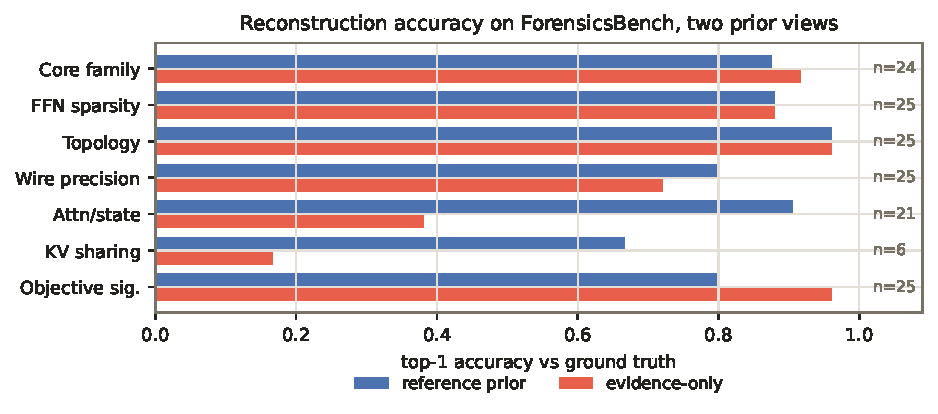
\includegraphics[width=.92\textwidth]{figures/fig_v4_accuracy.pdf}
\caption{Per-property top-1 accuracy under the reference prior (blue) and the
evidence-only flat prior (red).  The two views disagree exactly where a strong prior
meets a single decisive channel (core family, attention/state).}
\label{fig:accuracy}
\end{figure}

\subsection{The generation contract and the family split}
\label{sec:familysplit}
The generation test establishes what we call the \emph{autoregressive-compatible
generation contract}.  It looks at three things: how long a continuation the model
produces, whether latency grows with output length, and how finely the stream is
chunked.  This is deliberately a claim about the contract, not the architecture.  A
serving wrapper that returns at most one token per request could produce the same
observations with no autoregressive model behind it.  So the architecture-level reading
inherits that caveat, and the transformer-versus-SSM split below is what carries the
architecture-level discrimination.  Across \benchname{} the contract row is correct on
\FamilyPathAcc{} subjects, including both Mamba SSMs.  That is as it should be: SSMs
\emph{are} autoregressive at the contract level.  Our earlier draft featured a
``decoder-only 0.97'' score that silently blurred this distinction.  On the benchmark
that score is exactly as uninformative as a sceptical reviewer would expect, because
both SSM subjects score it too.

Telling a transformer from an SSM needs a different observable: the \emph{decode state}.
A transformer keeps a key-value cache that grows with every token, so each new token
costs slightly more time than the last.  An SSM keeps a state of fixed size, so the
per-token time stays flat.  The decode-state probe (P23) measures this slope from
streaming per-token times at contexts of 64 to 2048 tokens, which is inside every
deployment cap, taking the per-length minimum to suppress interference from other
tenants.  On \benchname{} the split is \SsmSplitAcc{} of the \SsmEligible{} eligible
subjects, meaning the causal, non-router ones.  The remaining six of 25 are structurally
ineligible: 4 encoders, the encoder-decoder, and the router (Fig.~\ref{fig:attncontrol}).
On the same-hardware control it separates full attention (+18.6\,\textmu s per token
per 1k of context, CI [16.3, 21.1]) from a 256-token sliding window (+1.8 [1.1, 2.6])
and from Mamba (+0.5 [$-0.0$, 1.2]).  We ran 60 trials per arm; only 3 were needed for
80\% power.  Two honest qualifications.  (i) Under the reference prior the categorical
call lags behind the evidence.  The prior odds against an SSM are 12 to 1, so a single
decisive channel moves SSM to top-1 only in the evidence-only view.  We show both.
(ii) On production endpoints with high serving overhead the channel is drowned in noise
at the spans we can reach, and there the probe abstains rather than guessing
(Sec.~\ref{sec:production}).

\begin{figure}[t]\centering
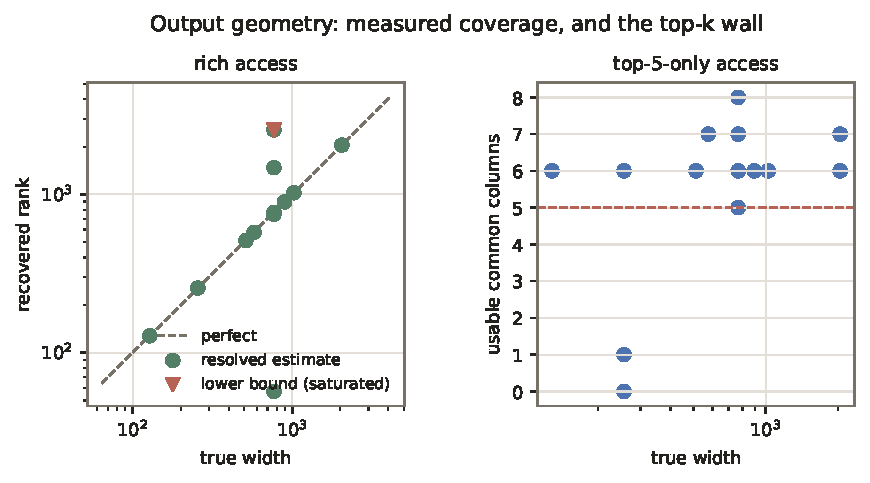
\includegraphics[width=\textwidth]{figures/fig_v4_geometry.pdf}
\caption{Left: recovered output-bottleneck rank against true width under rich access.
The adaptive ladder resolves widths up to 2{,}048 and reports lower bounds when it
saturates.  The visible off-diagonal cases are serving-axis artifacts, discussed in the
text: int8 quantisation deflates the measured rank (57 against a true 768), bf16 wire
rounding inflates it (2552 against 768), and the two-checkpoint router roughly doubles
it (1478).  The geometry channel detects the routing fixture that the topology prior
misses.  Right: under top-5-only access the usable common column set is a handful.  The
rank is capped by the observed columns (Prop.~\ref{prop:rank}), so width stays
unresolved.}
\label{fig:geometry}
\end{figure}

\subsection{Output geometry: coverage by width, and the top-\emph{k} wall}
\label{sec:geometry}
With the rich selected-column channel, the geometry protocol now \emph{adapts the
number of prompt rows to the width it is looking for}.  The ladder runs from 384 to
2560 rows, with a fixed relative threshold of $10^{-6}$ and a resolution gate fixed
before measurement.  The result is resolved estimates at widths \GeomResolvedList{},
which covers every core subject from 128 through 896, the 1{,}024-wide subject, and both
2{,}048-wide subjects, with relative errors under \GeomMaxErr{}, and lower bounds beyond
that.  At width 2{,}048 the ladder saturates at its 2{,}560-row cap and yields a lower
bound rather than a point estimate.  We report the bound.  Under the
production-realistic top-5-only regime, \emph{no} subject resolves.  The natural top-5
column union spans only \TopFiveCols{} columns on average, so the matrix rank is capped
by construction.  That is Prop.~\ref{prop:rank} made empirical.  This is the honest shape
of the claim: \textbf{width recovery is a budgeted capability that depends on the access
regime and comes with a measured coverage curve.  It is not a demo.}

\subsection{Numeric regime, tokenization, sparsity}
The wire-grid detector scores \DtypeAcc{} across the dtype variants (fp32, bf16, and
fp16 compute, plus the bf16-rounded wire).  The int8-dynamic case reads as a continuous
grid.  That is correct at the wire layer, and it is a documented limit on inferring the
compute dtype.  Tokenizer count-family matching is \TokenizerAcc{} exact within the
reference registry.  The domain-timing MoE detector is the weakest instrument, at
\MoeAcc{} top-1: small dense models served on CPU produce MoE-like timing signatures
often enough to matter.  We therefore report MoE on production \emph{at that measured
reliability}, and the interleaved-control follow-up (Sec.~\ref{sec:production}) replaces
the domain-timing signal where it matters.  The \emph{objective signature} row of
Table~\ref{tab:accuracy} measures the observable generation or masking contract (causal
versus masked versus prefix behaviour), not the historical training recipe.
Post-training can rewrite behaviour without touching the weights, so this row is named
and graded as a signature, never as a recovered training objective.

\paragraph{The prior/evidence gap is a measurement.}
The attention/state property scores \AttnRefAcc{} under the reference prior but only
\AttnFlatAcc{} under the evidence-only flat prior.  That is the largest prior-dependence
anywhere in the benchmark.  It is not merely a caveat.  It is a result about forensic
inference under weak channels: where the observable channel is thin (short-span recall
plus a noise-limited decode slope), confidence in an architectural property is driven
mostly by the structural prior.  The honest report is the pair of numbers, not either one
alone.  We report both views for every property precisely so that prior-driven support
is visible as such (Table~\ref{tab:accuracy}).

\begin{figure}[t]\centering
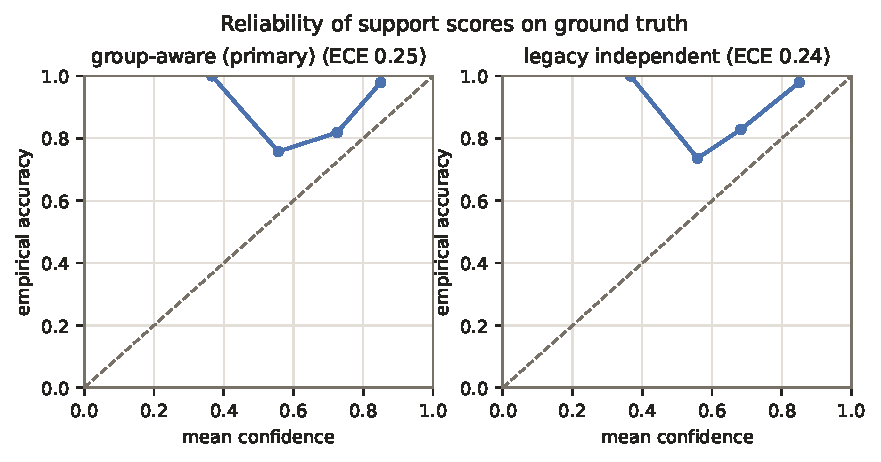
\includegraphics[width=.9\textwidth]{figures/fig_v4_reliability.pdf}
\caption{Reliability of support scores against \benchname{} ground truth: group-aware
ranker (left) versus the legacy independent-factor ranker (right).}
\label{fig:reliability}
\end{figure}

\subsection{Calibration: are the support scores honest?}
\label{sec:calibration}
Table~\ref{tab:calibration} reports the Brier score and ECE of the scores shown in this
paper, computed on \benchname{} labels, for the group-aware ranker (primary) and the
legacy independent-factor ranker (sensitivity).  The seven properties differ in how
many classes they have, how balanced those classes are, and how hard they are, so a
single pooled number would mix unlike prediction problems.  We therefore report the
\emph{macro-average} over properties with a property-bootstrap CI (ECE \BenchECE{}
\BenchECEMacroCI{}, Brier \BenchBrier{} \BenchBrierMacroCI{}) and the per-property values
in Table~\ref{tab:accuracy}.  Grouping protects against mechanically compounding
repeated evidence, which is the failure mode that motivated it.  But it does \emph{not}
improve these aggregate calibration metrics here (legacy: ECE \BenchECELegacy{}
\BenchECEMacroLegacyCI{}, Brier \BenchBrierLegacy{} \BenchBrierMacroLegacyCI{}).  We
report both schemes and claim no calibration improvement.  Scores remain support ranks,
never probabilities, and their rank order now carries a measured error rate per
property (Table~\ref{tab:accuracy}).

\begin{table}[h]\centering\small
\caption{Calibration of the support scores on \benchname{} ground truth,
macro-averaged over the seven heterogeneous properties of Table~\ref{tab:accuracy}
(each weighted equally, since their class counts and difficulties differ; CIs by
bootstrap over properties).  Per-property values appear in Table~\ref{tab:accuracy}.}
\label{tab:calibration}
\begin{tabular}{@{}l c c c c@{}}
\toprule
\textbf{Ranker} & \textbf{Brier} & 95\% CI & \textbf{ECE} & 95\% CI\\
\midrule
group-aware (primary) & 0.348 & [0.272,0.429] & 0.249 & [0.153,0.351] \\
legacy independent factors & 0.344 & [0.269,0.423] & 0.244 & [0.153,0.346] \\
\bottomrule
\multicolumn{5}{@{}l@{}}{\footnotesize Macro-averaged over the seven properties of Table~\ref{tab:accuracy} (equal weights);}\\
\multicolumn{5}{@{}l@{}}{\footnotesize CI by bootstrap over properties; per-property values in Table~\ref{tab:accuracy}.}\\
\end{tabular}

\end{table}
